\documentclass[conference]{IEEEtran}
\IEEEoverridecommandlockouts
% The preceding line is only needed to identify funding in the first footnote. If that is unneeded, please comment it out.
\usepackage{cite}
\usepackage{amsmath,amssymb,amsfonts}
\usepackage{algorithmic}
\usepackage{graphicx}
\usepackage{textcomp}
\usepackage{xcolor}
\def\BibTeX{{\rm B\kern-.05em{\sc i\kern-.025em b}\kern-.08em
    T\kern-.1667em\lower.7ex\hbox{E}\kern-.125emX}}
\begin{document}

\title{Course Project Midterm Report\\

}

\author{\IEEEauthorblockN{Clayton Tucker}
\IEEEauthorblockA{\textit{COSC 325} \\
\textit{Ctrl Alt Delete}\\
Knoxville, US \\
ctucke24@vols.utk.edu}
\and
\IEEEauthorblockN{Todd Van Meter}
\IEEEauthorblockA{\textit{COSC 325} \\
\textit{Ctrl Alt Delete}\\
Knoxville, US \\
tvanmete@vols.utk.edu}
\and
\IEEEauthorblockN{3\textsuperscript{rd} Given Name Surname}
\IEEEauthorblockA{\textit{COSC 325} \\
\textit{Ctrl Alt Delete}\\
Knoxvile, US \\
email address or ORCID}
\and
\IEEEauthorblockN{4\textsuperscript{th} Given Name Surname}
\IEEEauthorblockA{\textit{COSC 325} \\
\textit{Ctrl Alt Delete}\\
Knoxvile, US \\
email address or ORCID}
}

\maketitle

\begin{abstract}
The purpose of predicting stock prices is to ...  This can be done by developing a machine learning program that trains itself on previous stock prices.  There exist many different learning models to predict the future of stocks, though many of them are not considered efficient enough.  The aim of this project is to take an existing learning model and further improve it using learning techniques such as ARIMA, Linear Regression, or Random forests.  For this article, we will be using an ARIMA with Long Short Term Based Memory.  We hope to improve it by..
\end{abstract}

\begin{IEEEkeywords}
ARIMA, Linear Regression, Random forest, Stock Price Prediction
\end{IEEEkeywords}

\section{Introduction}
The prediction of stock prices has long been a subject of interest for investors, financial analysts, and researchers. Accurate prediction of stock prices can provide valuable information for decision-making in trading and investment strategies. However, stock price prediction is inherently complex due to the volatile and dynamic nature of financial markets. This project focuses on time series analysis to predict stock prices, specifically using historical stock data from Berkshire Hathaway Inc.

\subsection{Problem Overview}
Stock prices are influenced by a multitude of factors, including market trends, economic indicators, investor sentiment, and company performance. Traditional methods for predicting stock prices, such as fundamental and technical analysis, have limitations, as they rely on historical patterns and market assumptions. With advances in machine learning and deep learning, data-driven models have emerged as powerful tools for time series forecasting.

Subject to change.

In this project, our objective is to predict stock price movements using historical data consisting of features such as open price, close price, high and low prices, and trading volume. By analyzing these patterns over time, we seek to develop a model that can identify trends and potential future stock price fluctuations for Berkshire Hathaway. The unpredictability of the stock market poses challenges, but through proper analysis and appropriate modeling techniques, we can aim to improve prediction accuracy and offer valuable insight.

\subsection{Importance of Solution}
Accurate stock price prediction has significant implications for both individual and institutional investors. A reliable forecasting model can help investors make informed decisions, optimize portfolio management, and reduce financial risks. In addition, stock prediction models can contribute to the broader financial industry by enhancing risk assessment strategies and improving the trading algorithms used by hedge funds and financial institutions.

Berkshire Hathaway is a major player in the global financial market with a diverse portfolio of subsidiaries in multiple industries. Understanding and predicting the stock price movements of such a company can provide insight into broader economic trends and market behavior. Given Berkshire Hathaway’s substantial market capitalization and its influence on investment decisions around the world, an effective predictive model could have far-reaching applications. Investors, traders, and financial analysts could use such a model to make strategic decisions that align with market movements and economic conditions.

Moreover, stock price prediction is not only about maximizing financial gains, but also about mitigating losses. Market volatility can lead to substantial financial risks, and an improved prediction model could help investors develop risk management strategies to protect their investments. By reducing uncertainty, investors can make data-driven decisions rather than relying on speculation or intuition.

\subsection{Project Goal}
The primary objective of this project is to develop a stock price prediction model using historical stock data from Berkshire Hathaway. Our goal is to explore various time series forecasting techniques, including statistical models and machine learning approaches, to determine the most effective method for predicting stock price trends. The analysis will focus on leveraging features such as open, close, high, low prices, and trading volume to train the model.

Through this research, we aim to achieve the following:
\begin{itemize}
\item Investigate the effectiveness of different time series prediction models for stock price forecasting.

\item Evaluate the impact of various stock price features on prediction accuracy.

\item Develop a predictive model that can provide insights into future stock price movements with a reasonable degree of accuracy.

\item Provide an in-depth analysis of the results and discuss potential applications and limitations of the model.

\item Assess the feasibility of using machine learning techniques in financial forecasting and their implications for the stock market.
\end{itemize}

By accomplishing these goals, we hope to contribute to the growing field of financial analytics and offer valuable insights for investors and analysts looking to enhance their decision-making processes in stock trading. This project will not only serve as an academic exploration of time series forecasting but also provide practical implications for real-world financial markets.

In summary, the study of stock price prediction using historical data is an essential aspect of financial analytics. With the increasing role of technology in market analysis, leveraging advanced machine learning and statistical techniques can enhance our ability to forecast market trends accurately. This research will help bridge the gap between traditional financial analysis and modern predictive modeling, offering valuable contributions to the field of financial forecasting and investment strategy.


\section{Data Exploration}

 Discuss the dataset for this project, any cleaning and normalization steps, and any trends and insights about the dataset (i.e., exploratory data analysis (EDA)).

 \subsection{Cleaning and Normalization}
Ask what they did with the data

Put in a picture of how our data is stored

\includegraphics[scale=0.5]{example-image.jpg}


 \subsection{Trends and Insights}
 To make sure ARIMA works properly, we remove trends and make the data more stationary.
 Ask for any insights

\section{Baseline Model}

Many different baseline models to choose from.  Elaborate on the choices

\subsection{Existing Solutions: }

WE SHOULD ADD SOME FIGURES HERE

\begin{itemize}
\item{Linear Regression: }
Used for predicting continuous values given independent values.  Such factors we can consider using for this model would be low, open, high, close, or volume.  There is a problem using linear regression, as data in stock prediction is typically nonlinear.
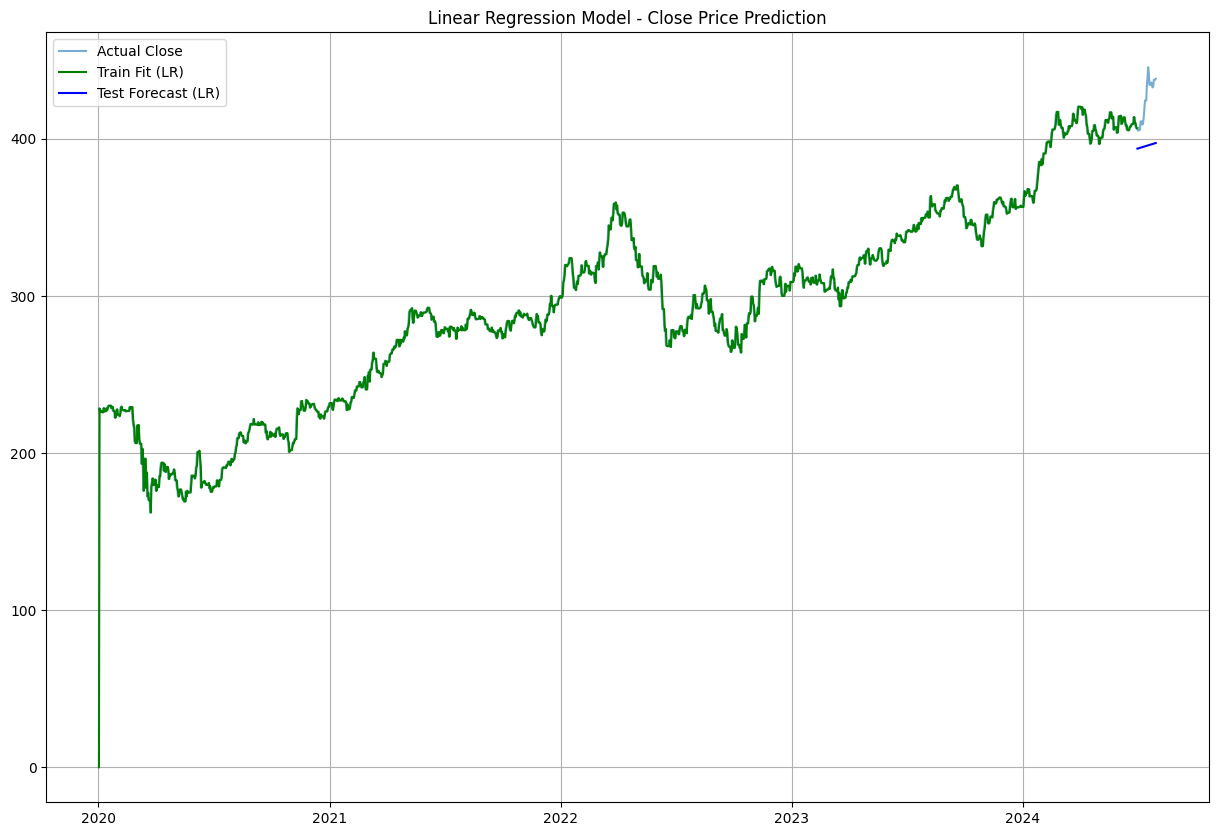
\includegraphics[scale=0.5]{screenshots/linreg.png}

\item{Random Forest: }
A Random Forest model does...  Benefits:  Negatives:
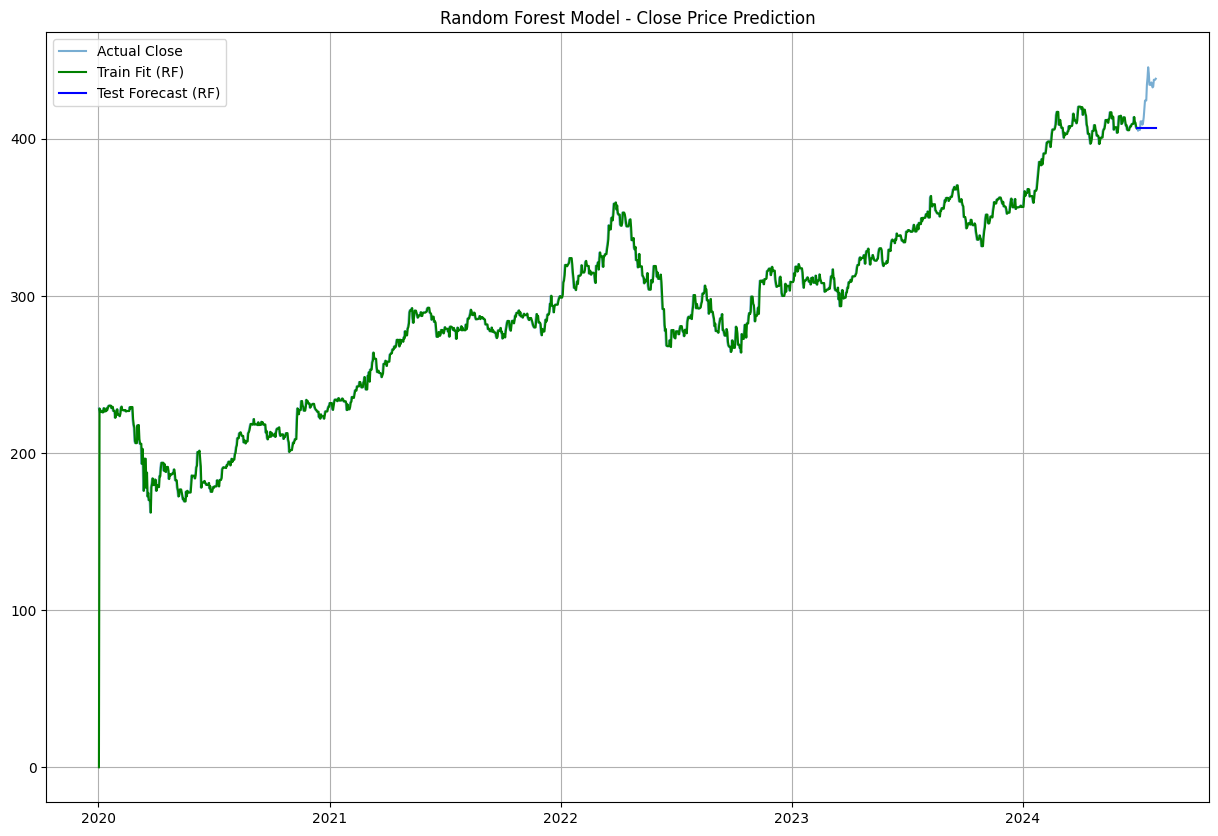
\includegraphics[scale=0.5]{screenshots/ranfor.png}

\item{Long Short Term Based Memory Model: }
An advanced version of the Recurrent-Neural-Networks (RNN), where previous information is used in training.  
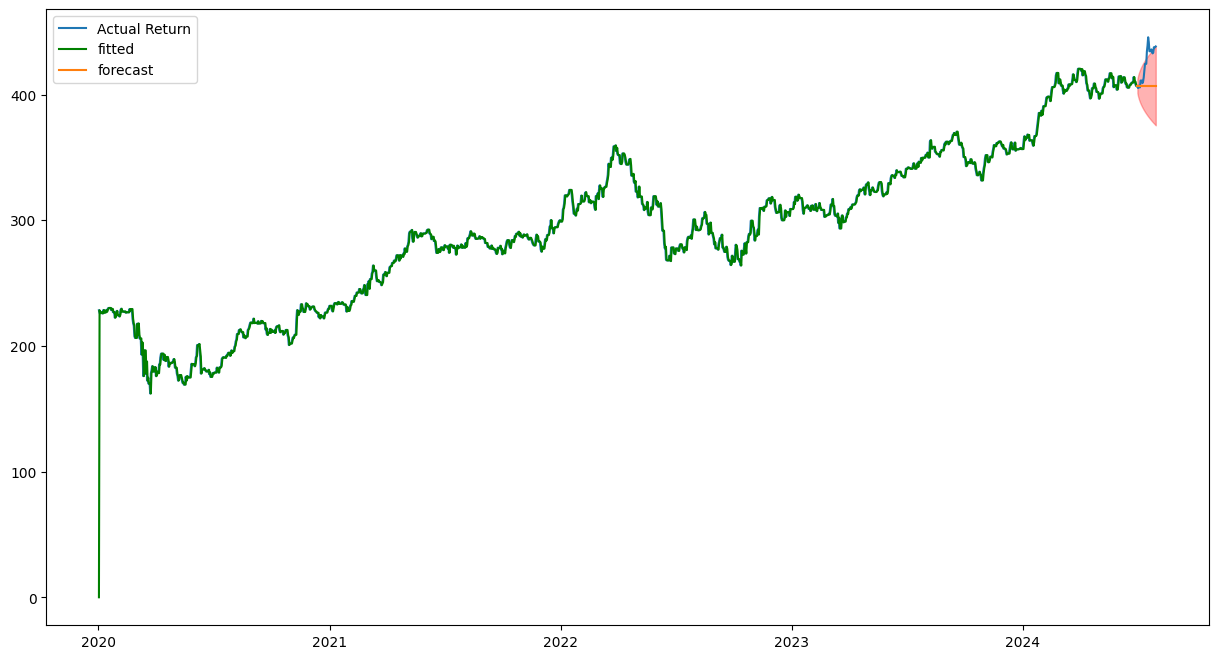
\includegraphics[scale=0.5]{screenshots/arima.png}

\end{itemize}

\subsection{Selection of Baseline}
We chose to use an ARIMA with a Long Short Term Based Memory model as our baseline for this project.

\subsection{Baseline Performance}
Here is the data of the baseline, import a picture of it running
\\
\includegraphics[scale=0.5]{example-image.jpg}

\subsection{implementation}
ASK how to implement and what was done

\section{Improvements}
Traditional indicators: Using moving averages, RSI, and MACD do not effectively capture nonlinear relationships between data.

Propose enhancements to the machine learning pipeline, such as new feature engineering, baseline model improvements, and or visualization.




\begin{thebibliography}{00}
\bibitem{b1} G. Eason, B. Noble, and I. N. Sneddon, ``On certain integrals of Lipschitz-Hankel type involving products of Bessel functions,'' Phil. Trans. Roy. Soc. London, vol. A247, pp. 529--551, April 1955.
\bibitem{b2} J. Clerk Maxwell, A Treatise on Electricity and Magnetism, 3rd ed., vol. 2. Oxford: Clarendon, 1892, pp.68--73.
\bibitem{b3} I. S. Jacobs and C. P. Bean, ``Fine particles, thin films and exchange anisotropy,'' in Magnetism, vol. III, G. T. Rado and H. Suhl, Eds. New York: Academic, 1963, pp. 271--350.
\bibitem{b4} K. Elissa, ``Title of paper if known,'' unpublished.
\bibitem{b5} R. Nicole, ``Title of paper with only first word capitalized,'' J. Name Stand. Abbrev., in press.
\bibitem{b6} Y. Yorozu, M. Hirano, K. Oka, and Y. Tagawa, ``Electron spectroscopy studies on magneto-optical media and plastic substrate interface,'' IEEE Transl. J. Magn. Japan, vol. 2, pp. 740--741, August 1987 [Digests 9th Annual Conf. Magnetics Japan, p. 301, 1982].
\bibitem{b7} M. Young, The Technical Writer's Handbook. Mill Valley, CA: University Science, 1989.
\bibitem{b8}[1]I. Parmar et al., “Stock Market Prediction Using Machine Learning,” 2018 First International Conference on Secure Cyber Computing and Communication (ICSCCC), Dec. 2018, doi: https://doi.org/10.1109/icsccc.2018.8703332.
‌
\end{thebibliography}
\vspace{12pt}


\end{document}


